\hypertarget{sdk_overview_sdk_overview_introduction}{}\section{Introduction }\label{sdk_overview_sdk_overview_introduction}
Harman International Industries, Inc. has developed a software Protocol Stack to support Ethernet Audio Video Bridging (E\+A\+VB or A\+VB) on a variety of platforms. The software includes explicit Operating System and Hardware Abstraction Layers (O\+S\+AL and H\+AL) to facilitate rapid and efficient porting of the generic stack to specific platforms. The complete O\+P\+E\+N\+A\+VB E\+A\+VB implementation, and its role within an overall E\+A\+VB system are discussed in O\+P\+E\+N\+A\+VB?s Ethernet Audio Video Bridging (A\+VB) High Level Specification (O\+P\+E\+N\+A\+V\+B13-\/01059).

The O\+P\+E\+N\+A\+VB A\+VB stack is designed to work on both General Purpose O\+Ses (G\+P\+OS), such as Linux, as well as Real-\/\+Time O\+Ses (R\+T\+OS). There are some difference in concepts and terms between a G\+P\+OS and R\+T\+OS, for example threads vs tasks, or the concept of multiple processes. For the purposes of the S\+DK guides the terms thread and task are used interchangeably.

The guides in this S\+DK focus on integrating the O\+P\+E\+N\+A\+VB A\+VB stack in an application, developing interface module components and configuration A\+VB streams. These guides are separated into four sections\+:


\begin{DoxyItemize}
\item \hyperlink{sdk_overview}{E\+A\+VB S\+DK Overview}
\item \hyperlink{sdk_integration}{E\+A\+VB Integration}
\item \hyperlink{sdk_avtp_interface_module_dev}{A\+V\+TP Interface Module Development}
\item \hyperlink{sdk_avtp_stream_cfg}{A\+V\+TP Stream Configuration}
\end{DoxyItemize}

This overview section will cover general architecture.

~\newline
\hypertarget{sdk_overview_sdk_overview_glossary}{}\section{Glossary }\label{sdk_overview_sdk_overview_glossary}
{\bfseries A\+AF\+:} A\+V\+TP Audio Format

{\bfseries A\+VB\+:} Audio Video Bridging (used interchangeably with E\+A\+VB)

{\bfseries A\+VB Stack\+:} The primary functionality that implements the various A\+VB protocols

{\bfseries A\+V\+TP\+:} Audio Video Transport Protocol

{\bfseries E\+A\+VB\+:} Ethernet Audio Video Bridging (used interchangeably with A\+VB)

{\bfseries E\+M\+AC\+:} Ethernet Media Access Control

{\bfseries F\+Q\+T\+SS\+:} Forwarding and Queuing enhancements for Time Sensitive Streams

{\bfseries G\+P\+OS\+:} General purpose OS

{\bfseries g\+P\+TP\+:} generalized Precision Time Protocol

{\bfseries H\+AL\+:} Hardware Abstraction Layer

{\bfseries Listener\+:} Receives an A\+V\+TP stream, unpacks it and pushes it to a media sink for playback. It consists of a dedicated task and uses functionality in the A\+V\+TP module, one mapping module and one interface module.

{\bfseries I\+E\+EE\+:} Institute of Electrical and Electronics Engineers

{\bfseries Interface Module\+:} An A\+V\+TP component that when called from the talker pulls data from a media source and pushes it onto the media queue in the format expected by the mapping module running on the talker. When called from a listener it pulls data from the media queue and pushes it to the media sink for playback.

{\bfseries I\+SR\+:} Interrupt Service Routine

{\bfseries M\+A\+AP\+:} Multicast Address Allocation Protocol

{\bfseries M\+AC\+:} Media Access Control

{\bfseries Mapping Module\+:} An A\+V\+TP component that when called from the talker pulls data from the media queue and packages it into the A\+V\+TP data payload according to a specific A\+VB encapsulation. When called from a listener it unpacks the A\+V\+TP data payload according to the specific A\+VB encapsulation and pushes it on to the media queue.

{\bfseries Media Queue\+:} A circular F\+I\+FO container used to opaquely pass media data blocks between interface modules and mapping modules. This is the only way interface modules and mapping modules communicate.

{\bfseries M\+J\+P\+EG\+:} Motion Joint Photographic Expert Group

{\bfseries M\+P\+E\+G2-\/\+TS\+:} Motion Picture Expert Group (version 2) Transport Stream

{\bfseries OS\+:} Operating System

{\bfseries O\+S\+AL\+:} Operating System Abstraction Layer

{\bfseries S\+DK\+:} Software Development Kit

{\bfseries SR\+:} Stream Reservation

{\bfseries R\+T\+OS\+:} Real-\/time OS

{\bfseries S\+RP\+:} Stream Reservation Protocol

{\bfseries Stream\+:} A series of A\+V\+TP data packets

{\bfseries Talker\+:} Takes an audio or video source and transmits it as an A\+V\+TP stream on the A\+VB network. It consists of a dedicated task and uses functionality in the A\+V\+TP module, one mapping module and one interface module.

~\newline
\hypertarget{sdk_overview_sdk_overview_architecture}{}\section{Architecture }\label{sdk_overview_sdk_overview_architecture}
The complete O\+P\+E\+N\+A\+VB E\+A\+VB implementation and its role within an overall E\+A\+VB system are discussed in O\+P\+E\+N\+A\+VB?s Ethernet Audio Video Bridging (A\+VB) High Level Specification (O\+P\+E\+N\+A\+V\+B13-\/01059).

What follows in this section are details that more directly effect the use and understanding of the S\+DK.

~\newline


Below is the component diagram of the Core A\+VB stack. Notice that the interface modules are not shown as part of the formal core stack but instead the interfaces that they use in the core stack are shown. This is also true for the interfaces the host application will use (TL A\+P\+Is).


\begin{DoxyImage}
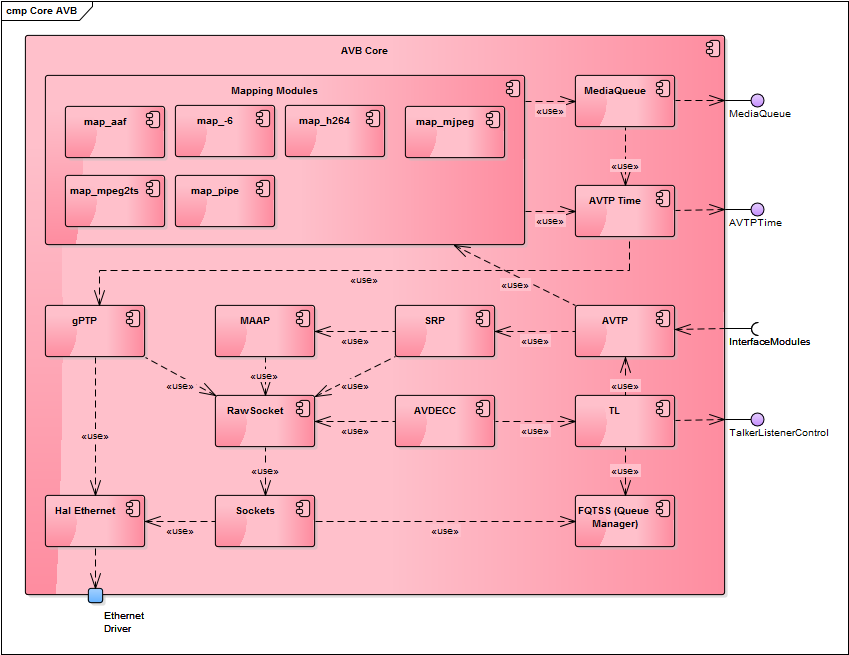
\includegraphics[width=15cm]{Core_AVB.png}
\caption{Core A\+VB}
\end{DoxyImage}


~\newline


General Purpose O\+Ses will generally have the core A\+VB stack split across multiple processes. Whereas in an R\+T\+OS everything sits within a single execution image. Here is a process diagram of the components split across processes in the Linux reference implementation.


\begin{DoxyImage}
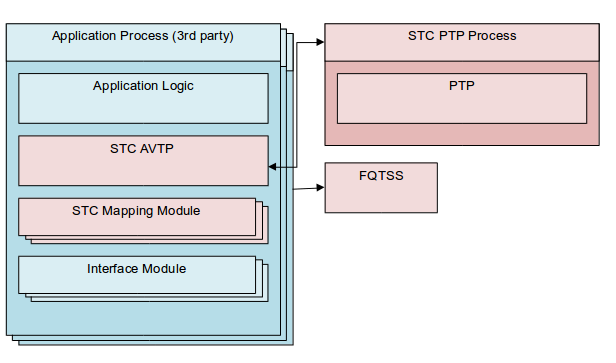
\includegraphics[width=15cm]{fig1.png}
\caption{A\+VB Components}
\end{DoxyImage}


As shown above the A\+V\+TP component of A\+VB is present in the application task. The A\+VB stack library gets initialized and loaded via the A\+P\+Is exposed and documented here. This static library implements that A\+V\+TP functionality as well as controlling talker and listener initialization and life cycle. The P\+TP task initialization is handled during stack initialization.

~\newline


The common A\+V\+TP stream data flow is shown here.


\begin{DoxyImage}
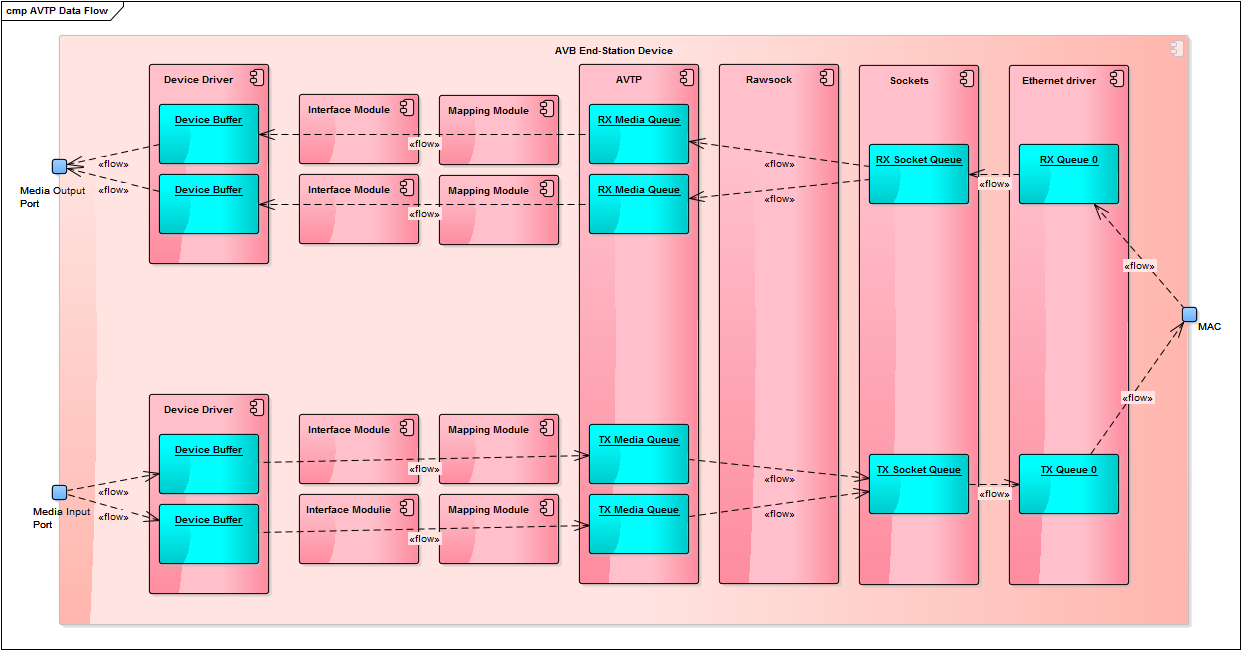
\includegraphics[width=15cm]{AVTP_Data_Flow.png}
\caption{A\+V\+PT Data Flow}
\end{DoxyImage}


~\newline


The diagram below shows an audio stream flowing through the A\+VB system on the Linux platform. Typically the talker and listener will be in different tasks and may use different interfaces.


\begin{DoxyImage}
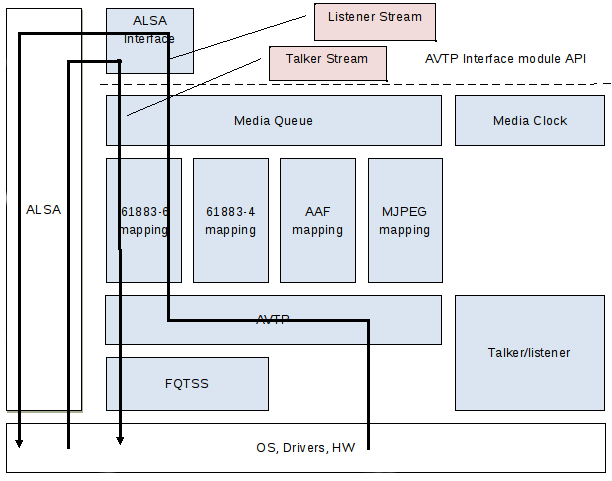
\includegraphics[width=15cm]{fig2.png}
\caption{A\+VB Audio Stream Flow}
\end{DoxyImage}


~\newline


Understanding the stream life-\/cycle is important for use of this S\+DK. Below are sequence diagrams that show the component interaction for key stream use cases.


\begin{DoxyImage}
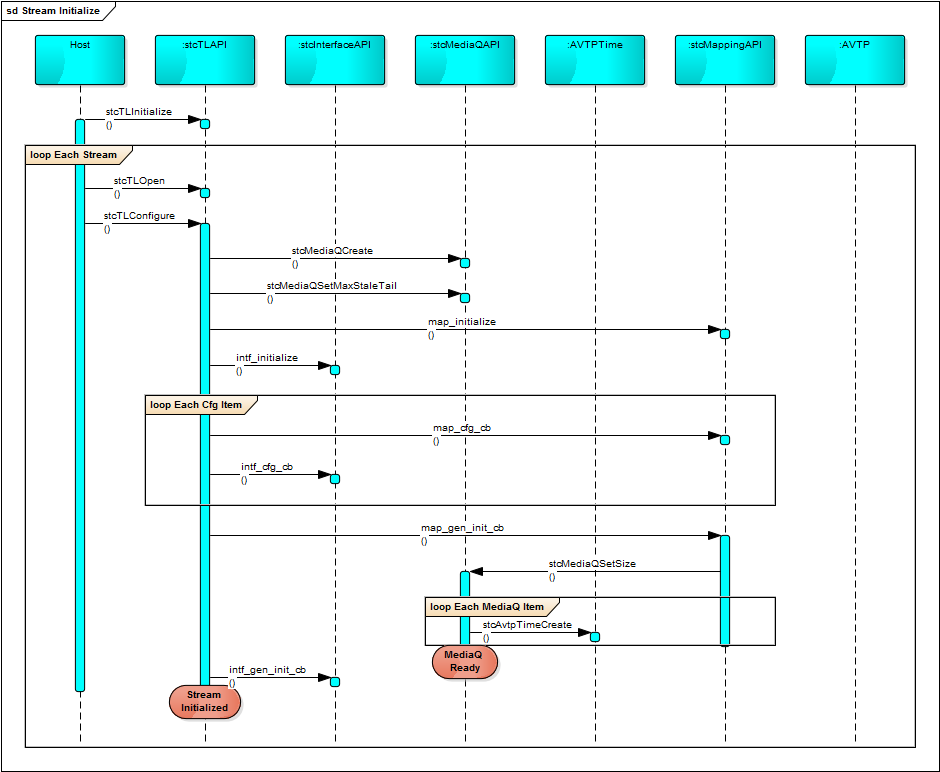
\includegraphics[width=15cm]{Stream_Initialize.png}
\caption{Stream Initialization}
\end{DoxyImage}


~\newline



\begin{DoxyImage}
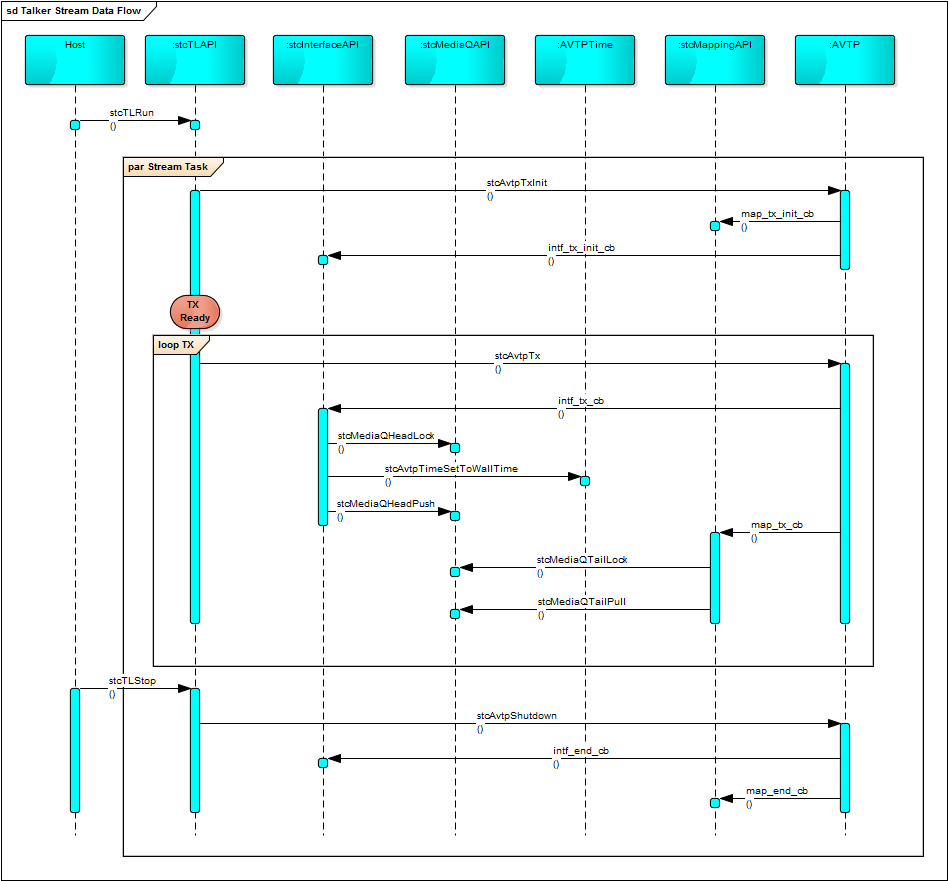
\includegraphics[width=15cm]{Talker_Stream_Data_Flow.png}
\caption{Talker Stream Data Flow}
\end{DoxyImage}


~\newline



\begin{DoxyImage}
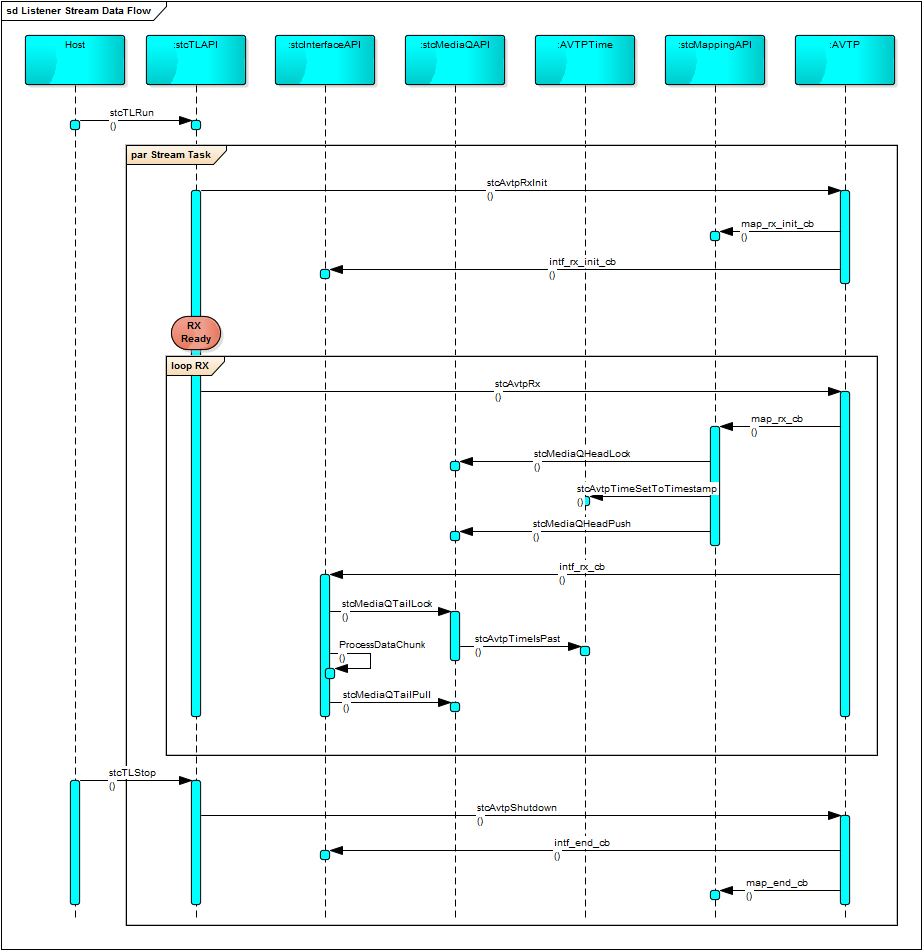
\includegraphics[width=15cm]{Listener_Stream_Data_Flow.png}
\caption{Listener Stream Data Flow}
\end{DoxyImage}


~\newline
\hypertarget{sdk_overview_sdk_overview_integration}{}\section{Integration, Extension and Configuration }\label{sdk_overview_sdk_overview_integration}
Three distinct uses of the S\+DK are as follows.

{\bfseries Integration\+:} This refers to the integration of the O\+P\+E\+N\+A\+VB A\+VB stack into an existing or new application. This is also sometimes referred to as the hosting application. For details related to this see \hyperlink{sdk_integration}{E\+A\+VB Integration}

{\bfseries A\+V\+TP Interface Module Development\+:} In order for the A\+VB stack to be used it must have interaction with media data sources and sinks on the platform. This is accomplished with Interface modules. The A\+VB stack ported to a platform may include some interface modules already but typically new interface modules are needed for the specific hardware and drivers being targeted. See \hyperlink{sdk_avtp_interface_module_dev}{A\+V\+TP Interface }Module Development" for more details.

{\bfseries Configuration\+:} Configuration can be split into 2 distinct area. Hosting application configuration and stream configuration. Hosting application configuration is port specifici and therefore not covered in detail in this S\+DK. However, in the configuration guide section of the S\+DK some host application configuration example are provided as a point of reference. The other primary area of configuration is related to stream. See the section \hyperlink{sdk_avtp_stream_cfg}{A\+V\+TP Stream }Configuration" for more details.

~\newline
\hypertarget{sdk_overview_sdk_overview_platform}{}\section{Platform Specific Considerations }\label{sdk_overview_sdk_overview_platform}
The O\+P\+E\+N\+A\+VB A\+VB stack is designed for portability covering both general purpose O\+Ses and real-\/time O\+Ses. The base public A\+P\+Is of the S\+DK do not change depending on the port. However, some elements of working with the S\+DK do change depending on the port of the O\+P\+E\+N\+A\+VB stack. See the release notes for the specific port for details that may be beyond the common S\+DK usage.

\subsection*{Threads / Tasks}

Within the S\+DK guides the terms threads and tasks are used interchangeability and for the purposes of the S\+DK they can be considered the same.

\subsection*{Processes}

Some platform O\+Ses support multiple processes. The O\+P\+E\+N\+A\+VB stack for a particular port may make use of multiple processes. For example in the Linux reference implementation g\+P\+TP resided in a separate process. Additionally in this reference implementation the talk / listener end-\/station functionality for each stream can be in a single process or split across multiple processes. Whereas in a R\+T\+OS there isn\textquotesingle{}t typically the concept of multile processes.

\subsection*{Configuration Overview}

Configuration of both the host application as well as the streams can vary based on platform capabilities. For example on configuration information may come from .ini files on the device and in other platforms there may not be a file system in which case configuration may be set at build time.

\subsection*{Startup}

See the port specific Release Notes for the details on A\+VB start up.

\subsection*{Libraries}

The A\+VB core stack commonly is build as a static library and linked with a hosting application. Interface modules may be built differently depending on the platform. In some cases they my be dynamic libraries and other cases they may be static libraries. It is also possible that the interface modules will be built with the host application or as part of the A\+VB core library. 